\documentclass[10pt]{article}
\usepackage{palatino}
\usepackage{fullpage}
\usepackage{latexsym}
\usepackage{amsfonts}
\usepackage{hyperref}
\usepackage{multicol}
\usepackage{fancyhdr}
\usepackage{enumitem}
\usepackage{caption}
\usepackage{subcaption}
\usepackage{fancybox}
\usepackage{framed}

\pagestyle{empty}                       %no page numbers
\thispagestyle{empty}                   %removes first page number
\setlength{\parindent}{0in}

\usepackage{fullpage}
\usepackage[tmargin = 0.5in, bmargin = 1in, hmargin = 1in]{geometry}     %1-inch margins
\geometry{letterpaper}
\usepackage{graphicx}
\usepackage{amssymb}

	\thispagestyle{empty}
	\renewcommand{\headrulewidth}{0.0pt}
	\thispagestyle{fancy}
	\lhead{Name: \underline{\hspace{1.5in}}}
	\chead{MTH 201: Calculus}
	\rhead{\framebox{\textbf{Grade: \ S \quad P}} }
	\lfoot{}
	\cfoot{}
	\rfoot{}


\begin{document}

	\vspace*{0in}

		\begin{center}
			\textbf{Learning Target C1 \\
			Version 6} \\
		\end{center}


\begin{framed}
	\textbf{C1: Compute the limit of a function at a specific point using the graph of the function. }
\end{framed}

Below is the graph of a function $f$. 

\begin{center}
    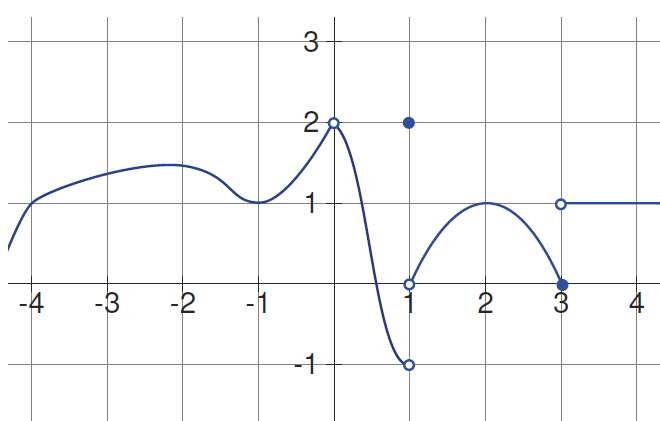
\includegraphics[width=4in]{limits-oct16.png}
\end{center}

State the value of each of the following limits. If the limit does not exist, state ``Does not exist''. You do not need to justify your answers, but all answers must be correct. 

\begin{enumerate}
    \item $\displaystyle{\lim_{x \to 0} f(x)}$
    \item $\displaystyle{\lim_{x \to 1} f(x)}$
    \item $\displaystyle{\lim_{x \to 3} f(x)}$
\end{enumerate}


\vfill


\begin{small}
    \begin{framed}
        	\textbf{Criteria for Satisfactory grade:} All limits are correctly stated.
    \end{framed}

\end{small}

\end{document}
